%%%%%%%%%%%%%%%%%%
% GitHub: A tool for social data set development and verification in the cloud
% Christopher Gandrud
% 15 January 2013
%%%%%%%%%%%%%%%%%

% !Rnw weave = knitr

\documentclass[twocolumn]{article}\usepackage{graphicx, color}
%% maxwidth is the original width if it is less than linewidth
%% otherwise use linewidth (to make sure the graphics do not exceed the margin)
\makeatletter
\def\maxwidth{ %
  \ifdim\Gin@nat@width>\linewidth
    \linewidth
  \else
    \Gin@nat@width
  \fi
}
\makeatother

\IfFileExists{upquote.sty}{\usepackage{upquote}}{}
\definecolor{fgcolor}{rgb}{0.2, 0.2, 0.2}
\newcommand{\hlnumber}[1]{\textcolor[rgb]{0,0,0}{#1}}%
\newcommand{\hlfunctioncall}[1]{\textcolor[rgb]{0.501960784313725,0,0.329411764705882}{\textbf{#1}}}%
\newcommand{\hlstring}[1]{\textcolor[rgb]{0.6,0.6,1}{#1}}%
\newcommand{\hlkeyword}[1]{\textcolor[rgb]{0,0,0}{\textbf{#1}}}%
\newcommand{\hlargument}[1]{\textcolor[rgb]{0.690196078431373,0.250980392156863,0.0196078431372549}{#1}}%
\newcommand{\hlcomment}[1]{\textcolor[rgb]{0.180392156862745,0.6,0.341176470588235}{#1}}%
\newcommand{\hlroxygencomment}[1]{\textcolor[rgb]{0.43921568627451,0.47843137254902,0.701960784313725}{#1}}%
\newcommand{\hlformalargs}[1]{\textcolor[rgb]{0.690196078431373,0.250980392156863,0.0196078431372549}{#1}}%
\newcommand{\hleqformalargs}[1]{\textcolor[rgb]{0.690196078431373,0.250980392156863,0.0196078431372549}{#1}}%
\newcommand{\hlassignement}[1]{\textcolor[rgb]{0,0,0}{\textbf{#1}}}%
\newcommand{\hlpackage}[1]{\textcolor[rgb]{0.588235294117647,0.709803921568627,0.145098039215686}{#1}}%
\newcommand{\hlslot}[1]{\textit{#1}}%
\newcommand{\hlsymbol}[1]{\textcolor[rgb]{0,0,0}{#1}}%
\newcommand{\hlprompt}[1]{\textcolor[rgb]{0.2,0.2,0.2}{#1}}%

\usepackage{framed}
\makeatletter
\newenvironment{kframe}{%
 \def\at@end@of@kframe{}%
 \ifinner\ifhmode%
  \def\at@end@of@kframe{\end{minipage}}%
  \begin{minipage}{\columnwidth}%
 \fi\fi%
 \def\FrameCommand##1{\hskip\@totalleftmargin \hskip-\fboxsep
 \colorbox{shadecolor}{##1}\hskip-\fboxsep
     % There is no \\@totalrightmargin, so:
     \hskip-\linewidth \hskip-\@totalleftmargin \hskip\columnwidth}%
 \MakeFramed {\advance\hsize-\width
   \@totalleftmargin\z@ \linewidth\hsize
   \@setminipage}}%
 {\par\unskip\endMakeFramed%
 \at@end@of@kframe}
\makeatother

\definecolor{shadecolor}{rgb}{.97, .97, .97}
\definecolor{messagecolor}{rgb}{0, 0, 0}
\definecolor{warningcolor}{rgb}{1, 0, 1}
\definecolor{errorcolor}{rgb}{1, 0, 0}
\newenvironment{knitrout}{}{} % an empty environment to be redefined in TeX

\usepackage{alltt}
\usepackage{fullpage}
\usepackage[authoryear]{natbib}
\usepackage[usenames,dvipsnames]{xcolor}
\PassOptionsToPackage{hyphens}{url}\usepackage{hyperref}
\hypersetup{
    colorlinks,
    citecolor=black,
    filecolor=black,
    linkcolor=cyan,
    urlcolor=cyan
}
\usepackage{dcolumn}
\usepackage{booktabs}
\usepackage{tikz}
\usepackage{todonotes}
\usepackage[utf8]{inputenc} 

%%%%%%% Title Page %%%%%%%%%%%%%%%%%%%%%%%%%%%%%%%%%%%%%%%%%%%%
\title{GitHub: A tool for social data set development and verification in the cloud}

\author{Christopher Gandrud \\
                {\emph{Yonsei University (Wonju) \& Hertie School of Governance}}\footnote{Lecture in International Relations \& Fiscal Governance Centre Fellow. Email: \href{mailto:christopher.gandrud@gmail.com}{christopher.gandrud@gmail.com}.}\footnote{The files used to create this article are available on GitHub at: \url{https://github.com/christophergandrud/PoliSciGitData}.}}

\begin{document}

\maketitle

A new data set is created. Analyses are run. An article is published. The data set languishes. The data set's creators move on to other projects. Maybe someone else accesses the data and updates it for their own work. However, these updates are never connected back to the original and the updates are not widely known about. So, multiple people end up wasting time making the same updates. Maybe another researcher finds a mistake in the original data set. They email the authors suggesting corrections. The original authors may or may not make the changes. If changes are made, there are no easily accessible records of them. Some researchers may even be reluctant to make their data available at all (partially) out of fear that someone may find a mistake and they will have to spend time making tedious corrections. 

These are all examples of ways that the development and management of social science data sets do not take advantage of knowledge distributed in the social science community. These problems are partially caused by the data storage tools social scientist use. Despite rapid recent advances in social technologies--Twitter, Facebook, and so on--the tools many social scientists use do not make it easy, nor do they provide incentives to collaboratively develop data sets and verify their accuracy, especially for people not involved in creating the original data set.

In this brief article I show that GitHub\footnote{\url{https://github.com/}} offers a comprehensive data storage service for social scientists creating and using original data sets. It has unique tools for \emph{social data set development and accuracy verification}. Furthermore, GitHub fits directly into an active research workflow, particularly one that also includes R.\footnote{GitHub can be used to store and develop entire social science research projects, not just data. However, I do not directly address these other topics here.}

GitHub was originally created and is widely used as a tool for software developers to work together on projects, especially open source projects, using the Git\footnote{\url{http://git-scm.com/}} version control system. It has been called the ``Facebook of programmers'' \citep{Xie2011}. Though GitHub is already often used by social scientists for statistical package development\footnote{For example the \emph{Zelig} R package \citep{Zelig2008,R-zelig} is hosted on GitHub. See \url{https://github.com/IQSS/Zelig}.} it initially seems strange for me to suggest that this service would be useful for social scientists building and maintaining data sets. However, a software program and many social science data sets are fundamentally similar. \emph{They are collections of text files}. GitHub is a means of storing, version controlling, and collaborating on text files. So if a social scientist's original data is (a) in a \textbf{plain text format}, such as comma-separated values (CSV),\footnote{All major statistical programs as well as Microsoft Excel and Apple's Numbers can save and open files in plain text formats like CSV.} and (b) has accompanying variable description files also in a plain text format--e.g. TXT plain text or Markdown (MD),\footnote{\url{http://daringfireball.net/projects/markdown/}} they can take full advantage of GitHub's features for social data set development and verification.\footnote{See Bowers \citeyearpar[3]{Bowers2011} for a discussion of the advantages of storing research files in plain text format.}

In this article I begin by discussing the features that we want from a cloud service to store social science data: stable storage, version control, access, and collaboration. Then I examine how strong these features are in three methods widely used to store social science data. Though each method has its strengths, none of them encourage social data set development and verification.

A few brief notes before beginning: To get started with Git and GitHub see the GitHub Set Up page: \url{https://help.github.com/articles/set-up-git}. In this article I give examples of how to take advantage of GitHub using their website and from the command line. However, there are also very good graphical user interface (GUI) versions of GitHub for Mac and Windows (see GitHub's Set Up page for more information). I focus on GitHub, but you can also use other services that work with Git such as Bitbucket\footnote{\url{https://bitbucket.org/}} for some of the same things. Nonetheless, I discuss GitHub because it has a much more comprehensive set of features and is more widely used. Finally, the tools I discuss in this article are suitable for the small to medium size data sets common in social science. Much larger data sets often cannot be efficiently stored in plain text files. GitHub is not a suitable storage service for very large data sets.

\section{What do we need from a cloud data storage service?}

A cloud storage service for actively developed and used social science data needs to enable at least four things: \emph{stable storage}, \emph{version control}, \emph{access}, and \emph{collaboration}.\footnote{\cite{King2007} discussed eight ``requirements for effective data sharing''. His focus was on replication data sets for published results, rather than actively developing original data sets. His requirements, nonetheless largely overlap with mine here with the exception of ``authorization'' and ``legal protection''. I discuss these below.} Obviously a cloud storage service needs to be a stable and reliable platform for data storage. The service needs to include version control--similar to track changes in a word processing program--so that the development of the data set can be understood and researchers are able to revert to old versions (see \cite{Bowers2011}, \cite{Healey2011} and \cite{Fredrickson2011} for discussions of version control).  Data stored on it needs to be accessible to both coauthors and others who wish to reproduce analyses \citep{Fomel2009}, verify the data sets' accuracy, or use the data sets in new projects \citep{Kelly2006,King1995}. Another key part of access is that the storage service makes it easy to both develop and use data sets as part of researchers' workflows. Finally, a cloud data storage service should make collaboration easy. As long as there are no confidentiality or other strong reasons to limit access to a data set, collaboration should not be limited to coauthors. It should be possible to also collaborate with non-coauthors so that the data set can be improved by taking advantage of knowledge (and motivation) distributed throughout the social science community. Ideally, this social data set development and verification keeps data sets more up-to-date and more accurate. 

\section{Data storage: the social science status quo}

Social science data is currently often stored in three ways. It may be stored locally on a researcher's computer, on a general purpose cloud storage service such as Dropbox\footnote{\url{https://www.dropbox.com/}} or Google Cloud Drive,\footnote{\url{https://drive.google.com/}} or on a specialized research hosting service, notably Dataverse.\footnote{\url{http://thedata.org/}} Each of these data storage methods has their strengths in terms of stable storage, access, version control, and collaboration. Nonetheless each are lacking in at least one important way and none of them promote social data set development and verification.

\paragraph{Local storage}

Local storage--data sets saved on individual researchers' computers--is the least robust form of data storage currently used. It is not a very stable form of storage as anyone knows if they have lost all of their files when their computer died. Version control with Git or some other program is possible with locally stored data. However, if the version control files are lost along with the data, the data is lost. Researchers with access to the computer can easily access the data and use it in their workflow, but access by coauthors is limited. Access by non-coauthors is very cumbersome. Files must be emailed in response to individual requests. These files are not automatically updated with new versions of the data. Because access is limited to users of the computer the data is stored on, collaboration, especially by non-coauthors is extremely limited.

\paragraph{General purpose cloud storage}

Dropbox and other general purpose cloud storage services offer much more robust storage. These services generally work by syncing files stored on individual computers with those on cloud servers. Dropbox has a basic version control system. If you are using Dropbox for free, every time you save a file that version is stored and accessible for 30 days.\footnote{Old versions are stored for longer with paid accounts.} In addition you could use Git with a data set stored on Dropbox. Access is usually very easy. These services can be accessed via desktop programs, mobile apps, and websites. Because files stored on individual computers are automatically synced with cloud servers it is very easy to incorporate them into a workflow. General purpose cloud storage services also make it possible to share files and folders via URL links. Collaboration with coauthors is very easy because folders can be shared. This means that official collaborators (those given permission to make changes to the folder, i.e. write access) can easily change files in the folder and these changes are automatically synced for all users.\footnote{This can create problems if multiple authors are making changes to the same files at the same time. For a discussion of file conflicts see \cite{Fredrickson2011}.} However non-coauthors, without write access to the shared folder cannot easily suggest specific changes. They must email their suggestions to one of the researchers with write access. This is not much better than a situation with locally stored files.

\paragraph{Dataverse}

Many journals--Political Analysis for example--require data used in articles they publish to be uploaded to a specialized research data storage service like Dataverse. Dataverse is a stable form of storage. It does have some version control features. It saves each version that is uploaded to it. Old versions are downloadable. Dataverse is easily accessible for anyone with an internet connection. But it is difficult to access data as part of a research workflow, at least using the standard version.\footnote{It is possible to build a custom version of Dataverse with some R integration.} Unlike Dropbox, for example, there is no way to automatically update a data set on Dataverse. You have to point and click to upload data files for each version. It is difficult to access data directly from a statistical program such as Stata or R. The data needs to be downloaded by pointing and clicking and then loaded into these programs. Finally, it is difficult to collaborate using Dataverse. Changes to a data set must be uploaded to the site manually, then manually downloaded by collaborators. There are also no direct ways for non-coauthors to suggest changes.

Dataverse is very good for what it is designed to do: store a snapshot of a data set for replicating specific published results \citep{King2007}. It is uniquely strong among all of the storage options discussed here for providing journals with branded replication data set archives and has built in mechanisms for ensuring that a journal is legally protected and that data users have proper authorization \citep[177-179]{King2007}. However, it is difficult to use Dataverse to store and access data as part of an \emph{ongoing research workflow}. In addition it does not easily enable or incentivize social data set development and verification of its accuracy. 

\section{Data Storage on GitHub}

Though admittedly requiring a steeper learning curve, GitHub meets the four criteria for data set storage very well. In this section I will demonstrate how to use GitHub for data set storage, version control, access, and collaboration. Rather than giving a complete introduction, I focus on specific important aspects of each feature in Git and GitHub. In this section I give examples from a data set stored on GitHub. It is a data set of countries' Gallagher Electoral Disproportionality index across time that I put together from data used in Gallagher \citeyearpar[updated through 2011]{Gallagher1991} and \cite{Carey2011}. The data set and more information about it is available at: \url{http://christophergandrud.github.com/Disproportionality_Data/}.

\subsection{Storing and version control}

Version control is an integral part of how GitHub stores files. GitHub remotely stores files in what Git calls ``repositories", repos for short. You can think of repos as the folder containing a data set, including the data, description files, citation, copyright, and other legal information, as well as any source code used to create the data set. Repos could also include PDFs of papers where the data set was used and code for replicating the analyses in these papers. Git version controls files in repositories and GitHub hosts them remotely in the cloud.\footnote{Specifically, GitHub files are stored on Rackspace (\url{http://www.rackspace.com/}).} 

With a GitHub account you can store repositories for free on GitHub if they are in what GitHub calls ``public repositories". Anyone can see the contents of public repositories, including all previous versions.\footnote{Private repositories are available allowing only official contributors to see their contents. Private repos require a paid account.} Users can have an unlimited number of public repositories. There is a soft storage size limit of one gigabyte per repository. This should be more than enough for most social science data sets if they are stored in plain text formats. Each repository is given a webpage. Here is a portion of the Electoral Disproportionality repository's main page:

\begin{center}
	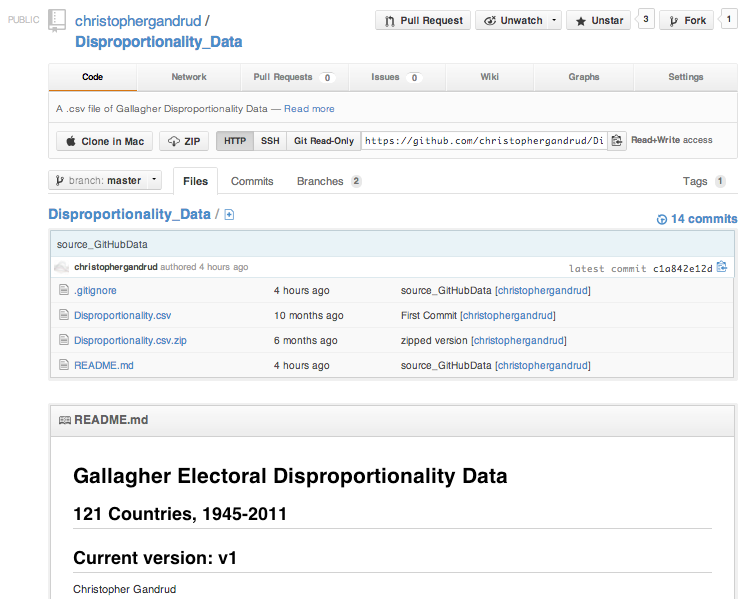
\includegraphics[width=0.46\textwidth]{images/MainPage.png}
\end{center}

Git is a very powerful version control system, especially for text files. For these types of files, Git only saves the actual changes when you (1) \texttt{add} a file to the repository and then (2) \texttt{commit} a version of the file to the repository. This is different from the other cloud storage services we have discussed. They save the whole file for each version. Each ``commit" in a repo is given a unique SHA-1 number identifying it. The author of the commit is also saved. Once you commit changes on your computer you can (3) \texttt{push} them to the remote GitHub version of the repo. A repo's GitHub website allows you to view all of the changes that have been made to it. You can browse all versions of the text files, view highlighted changes, and comment on these changes. For example:

\begin{center}
	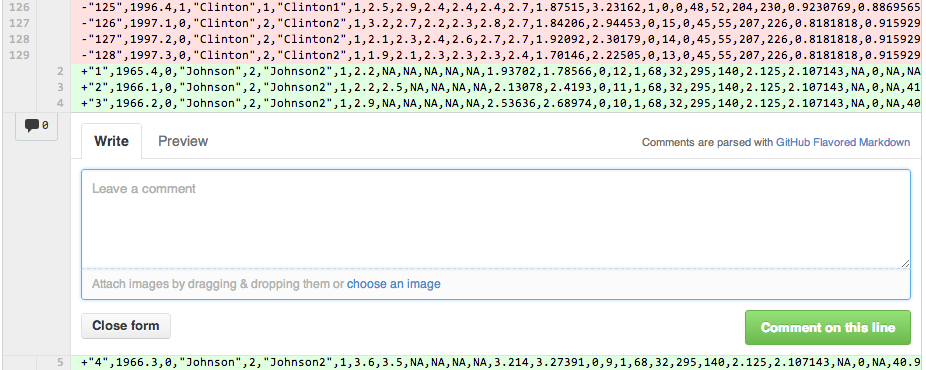
\includegraphics[width=0.46\textwidth]{images/BrowseChanges.png}
\end{center}

\noindent To see changes made to a file click on the \texttt{History} button located on the file's GitHub webpage.

\begin{center}
	
\includegraphics[width=0.4\textwidth]{images/Raw.png}
\end{center}

\noindent This will show the file's entire commit history. Click an individual commit's description to see and comment on the changes.

\paragraph{Contributor analytics}

An important component of version control on GitHub for us here is that because Git only commits changes and uniquely identifies the changer, it is possible to properly attribute every individuals' contribution to a data set. On the GitHub website you can see every change that has been made to each line of a file and who made the change. Git calls this ``blame''. To view who last changed each line of a file click on the \texttt{Blame} button on its GitHub page. It is next to \texttt{History}.

GitHub has graphical capabilities for organizing and displaying this data. One way to use these is by clicking on the \texttt{Graphs} button located near the top of each repository's webpage. This will give you access to graphs such as the ones below (I've blurred the contributors' names):

\begin{center}
	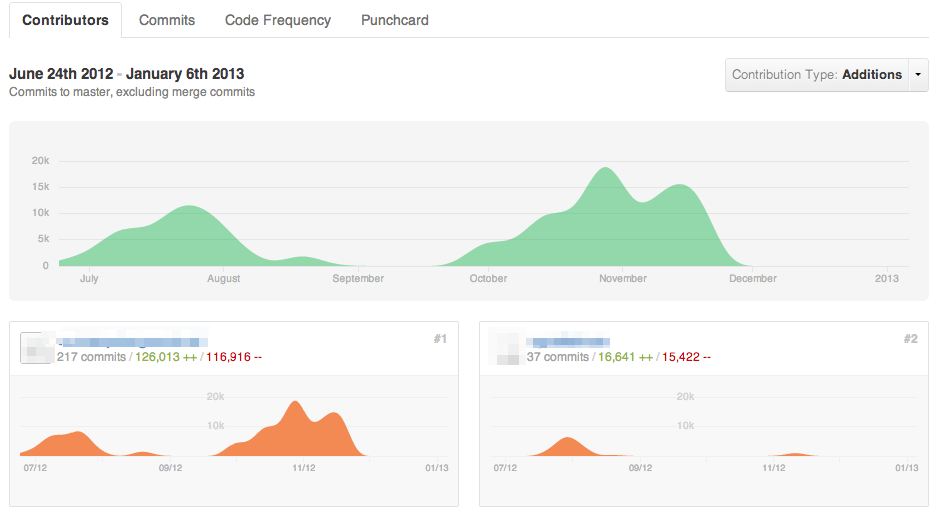
\includegraphics[width=0.46\textwidth]{images/CommitHistory.png}
\end{center}

\paragraph{Binary files}

I mentioned that Git treats non-plain text--binary--files differently. Stata's DTA data format and PDFs are examples of binary file types. Rather than committing specific changes, a new version of the entire binary file is stored with each commit \emph{if} they are changed. Binary files that are very very large can take up a lot of storage space when version controlled with Git.\footnote{Though it is important to note that previous commits are compressed, so the amount of storage space a committed binary file take up is less than the size of the original.} This is also a problem for all of the other data storage methods with version control discussed here. For very large binary files you will need to use a totally different type of cloud storage system like Rackspace or Amazon's S3.\footnote{\url{http://aws.amazon.com/s3/}} 

If you absolutely must have very large binary files in a repository one solution to the space constraints problem is to have Git ignore them. You do this by including a text file called .gitignore in the repository. In .gitignore simply type the binary file's name. Git will not version control it. This unfortunately also means that the file will not be pushed to GitHub.

\paragraph{Describe the data set with README files}

Each folder in a GitHub repository can contain a file called README.\footnote{Actually each folder in a repository can contain one as well.} README files for data sets can contain information about sources, variable descriptions, statements testifying that the collection and distribution of the data set violated no law, citation and copyright information, and so on. GitHub automatically displays the README file on the repository's website in full. If it is written in the Git Flavored Markdown\footnote{\url{http://github.github.com/github-flavored-markdown/}} mark-up language and called README.md, it will also be automatically formatted. You can see part of the Disproportionality data set's README.md above. 

\paragraph{Tagging versions}

Git can \texttt{tag} specific commits. Tags function as bookmarks for major versions of a Git repository. They are particularly useful for demarcating the version of a data set used in a particular publication, for example. Creating tags is simple. Imagine we want to tag the second major version of a data set, the one we used for a publication:

\begin{knitrout}
\definecolor{shadecolor}{rgb}{0.969, 0.969, 0.969}\color{fgcolor}\begin{kframe}
\begin{verbatim}
git tag -a v2 -m 'Citation Information'
\end{verbatim}
\end{kframe}
\end{knitrout}


\noindent The option \texttt{-a} means add, \texttt{v2} is the version number, and \texttt{-m} adds a message, in this case the publication's citation information. Now we simply \texttt{push} the tags to GitHub:

\begin{knitrout}
\definecolor{shadecolor}{rgb}{0.969, 0.969, 0.969}\color{fgcolor}\begin{kframe}
\begin{verbatim}
git push --tags
\end{verbatim}
\end{kframe}
\end{knitrout}


\noindent On GitHub there will be a list including the tag and an option to view and download this specific version of the data. For example:

\begin{center}
	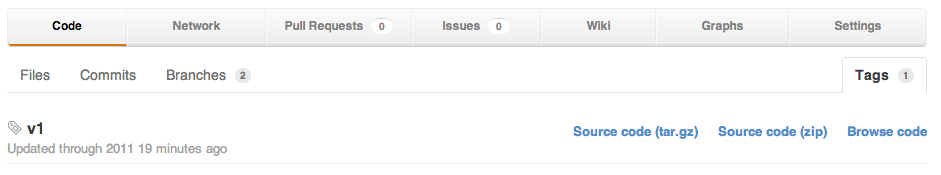
\includegraphics[width=0.47\textwidth]{images/GitTag.png}
\end{center}

\subsection{Accessing data}

There are many ways to access data stored on GitHub and incorporate it into your workflow. The simplest way is to use the GitHub website to actually edit files and commit changes. This can be handy for small changes, especially from mobile devices. As I mentioned, changes can also be committed on your computer and pushed to GitHub. You can use the command line version of Git or the GUI version of GitHub to push changes. RStudio,\footnote{\url{http://www.rstudio.com/}} a program that integrates R and mark-up languages like \LaTeX and Markdown, also includes Git and the ability to push a repo to GitHub. So it is possible to make changes to a repository, commit them, and push them to GitHub all within the same program. Here is a screenshot of this paper being written in RStudio. The Git functions are in the upper right pane. 

\begin{center}
	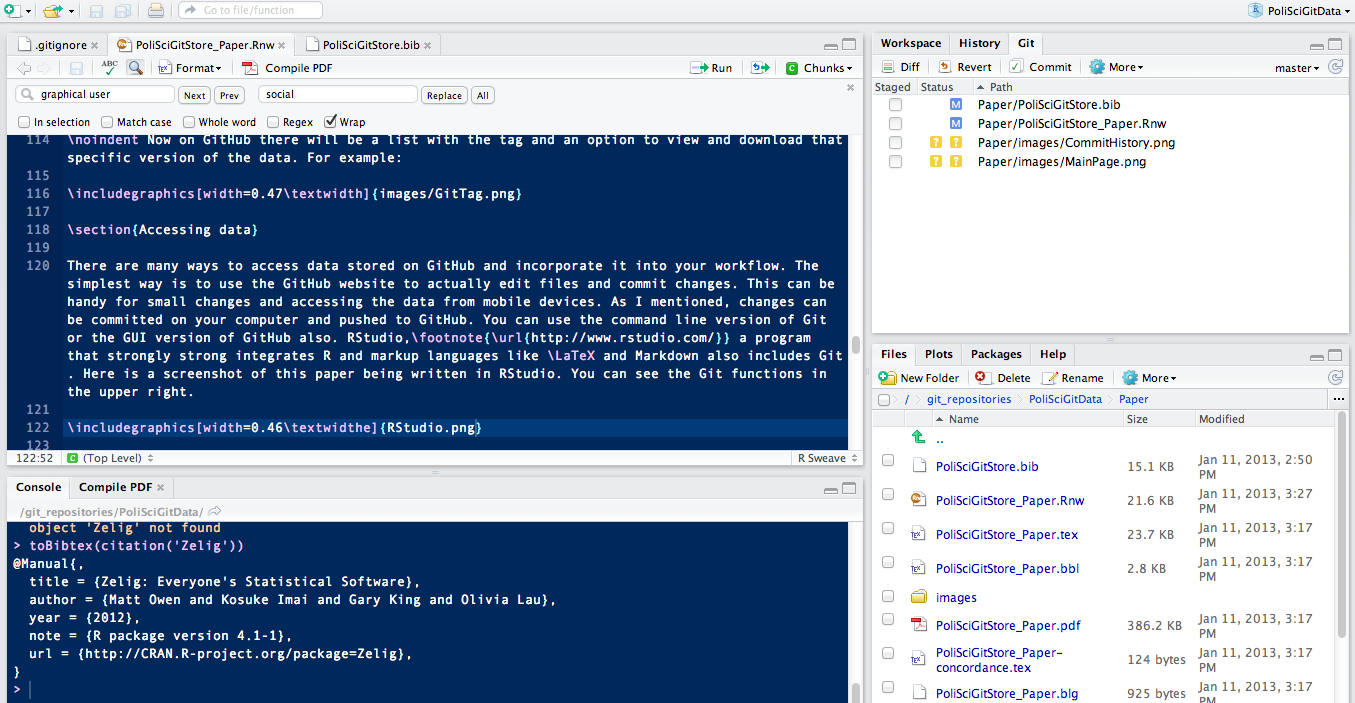
\includegraphics[width=0.46\textwidth]{images/RStudio.png}
\end{center}
\paragraph{Cloning a repo}

Repositories can be downloaded in full. This is called cloning. You can do this by clicking the \texttt{Clone in . . .} button on a GitHub repository's website. Cloning can also be done in the command line using a repository's address. For example, the Disproportionality data's clone-able address is: \url{https://github.com/christophergandrud/Disproportionality_Data.git}. 

{\small
\begin{knitrout}
\definecolor{shadecolor}{rgb}{0.969, 0.969, 0.969}\color{fgcolor}\begin{kframe}
\begin{verbatim}
git clone https://github.com/christophergandrud/
  Disproportionality_Data.git
\end{verbatim}
\end{kframe}
\end{knitrout}

}

\noindent Note that in real life the address needs to be on the same line. Also, before cloning a repository remember to change the working directory to the folder where you want to save it. In the command line use the \texttt{cd} command to do this.

Once you have cloned the repository you can role back to any previous version with the \texttt{checkout} command. For example if you want to roll back to a tag called ``v2", type:

\begin{knitrout}
\definecolor{shadecolor}{rgb}{0.969, 0.969, 0.969}\color{fgcolor}\begin{kframe}
\begin{verbatim}
git checkout v2
\end{verbatim}
\end{kframe}
\end{knitrout}


\noindent If you have permission to make changes to the repository (see below) you can then push any changes you make back to GitHub.

\paragraph{Access data directly from R}

Loading data stored on GitHub into R for use in statistical analysis is very easy.\footnote{You can of course also load data stored on the version of the repo located on your computer.} I have created a function that loads plain text formatted data from GitHub into an R data frame ready for analysis.\footnote{The function is based on \emph{devtools}' \texttt{source\_url} command.} It's called \verb|source_GitHubData| and is stored in a GitHub Gist\footnote{Gists host code snippet. See: \url{https://gist.github.com/}.} at: \url{https://gist.github.com/4466237}. It can be loaded into R using the \verb|source_gist| command from the \emph{devtools} package \citep{R-devtools}.

\begin{knitrout}
\definecolor{shadecolor}{rgb}{0.969, 0.969, 0.969}\color{fgcolor}\begin{kframe}
\begin{alltt}
\hlcomment{# Load source_GitHubData}
\hlcomment{# The functions' gist ID is 4466237}
devtools::\hlfunctioncall{source_gist}(\hlstring{"4466237"})
\end{alltt}
\end{kframe}
\end{knitrout}


\noindent The main argument in \verb|source_GitHubData| is \texttt{url}. You set this as the URL for the \emph{raw} version of plain text data file you want to download. The raw version is the version with only the text file. You find this URL by clicking the \texttt{Raw} button on the file's GitHub page. It's next to the \texttt{Blame} button we saw earlier. If you use the URL for the most recent commit of the file, you will always download the most recent version whenever you use \verb|source_GitHubData|. The raw URLs for each commit and tagged versions of the data are also accessible if you want to use a particular version. 

The URL for the raw version of the Electoral Disproportionality data is \url{http://bit.ly/Ss6zDO}.\footnote{I used bitly (\url{http://bitly.com/}) to shorten the URL so that it would fit on the page more easily. The full URL is: \url{https://raw.github.com/christophergandrud/Disproportionality_Data/master/Disproportionality.csv}.}  To download the data and put it in a data frame object called \emph{Data} using \verb|source_GitHubData| type:

\begin{knitrout}
\definecolor{shadecolor}{rgb}{0.969, 0.969, 0.969}\color{fgcolor}\begin{kframe}
\begin{alltt}
\hlcomment{# Download data}
Data <- \hlfunctioncall{source_GitHubData}(
          url = \hlstring{"http://bit.ly/Ss6zDO"})
\end{alltt}
\end{kframe}
\end{knitrout}


\noindent Note that by default \verb|source_GitHubData| loads CSV data. You can add the argument \verb|sep = "\t"| for tab-separated (TSV) data files. You can also specify \texttt{header = TRUE} (default) or \texttt{header = FALSE}.

\paragraph{Citing GitHub data}

When a researcher uses data they accessed via GitHub how can they cite it? A common practice for citing data is to cite the publication the data set was originally used in. However, this is incomplete in at least two ways. First, the version of the data used in the original publication may be different from that used later on. Second, it would be difficult to use this citation to acknowledge contributions made by contributors who did not work on the original data set, but contributed to later versions. One solution is to use the standard set by \cite{Altman2007} \citep[see also][183-184]{King2007}.\footnote{Dataverse uses a version of this standard.} They propose that data set citations have:

\begin{itemize}
  \item the author's name, 
  \item the date,
  \item the data set's title,
  \item a unique global identifier (UGI),
  \item a universal numeric fingerprint (UNF),
  \item a bridge service.
\end{itemize}

\noindent The first three are self explanatory and shared with standard citations for other types of materials. Examples of UGI include Document Object Identifiers (DOI)\footnote{http://www.doi.org/} and the Handel System.\footnote{\url{http://www.handle.net/}} They uniquely identify the data set. UNF's uniquely number a particular version of the data set. A bridge service allows you to use the DOI and UNF to link to the actual data set. Most UGI include a bridge service and create UNFs. One place to register DOIs for free (with restrictions) is the German National Library for Science and Technology.\footnote{\url{http://datacite.org/TIB}} 

You can use \citeauthor{Altman2007}'s citation standards to cite specific versions--tags and commits--of a data set stored with Git on GitHub. Citation information can be displayed on the version's README.md file. This allows you to persistently cite the exact version of the data set you used to achieve a particular result. Because Git stores information about each contribution it is possible with this citation method to identify every person who has contributed to a particular version of a data set and exactly what their contribution was.

\paragraph{Copyright and open data}

If you are creating an original data set that you want to and can--e.g. there are no confidentiality issues--make open while retaining authorship and enabling collaboration, it is worth considering how you want to copyright the data set.\footnote{Note that raw facts in a data set cannot be copyrighted, though the present layout and procedures used to gather the data can \citep[39]{Stodden2009}.} Any copyright information can be placed in a repository's main README.md file. This is a common practice for open source software stored on GitHub. For discussions of why and how to copyright data see \cite{Stodden2009} and \cite{CreativeCommons}.

\paragraph{Showcase a data set with GitHub Pages}

Each public repository's GitHub website allows anyone full access to the data. However, these pages may be confusing for those without experience using a version control system. To solve this problem GitHub Pages\footnote{\url{http://pages.github.com/}} allows you to very easily create a simpler display webpage for the repository. These pages can be used to describe the data and include links to download the entire repository. You can of course also add links to specific files.

To create a page navigate to the repository's normal GitHub webpage. Then click \texttt{Settings} \textrightarrow{} \texttt{Automatic Page Generator}. By default it will load the README file as the content of the new page. You can change this, add a Google Analytics tracking ID\footnote{\url{http://www.google.com/analytics/}} to gather information on who visits the page, and choose an aesthetic style before publishing it. Here is a sample of the Disproportionality data's page:

\begin{center}
	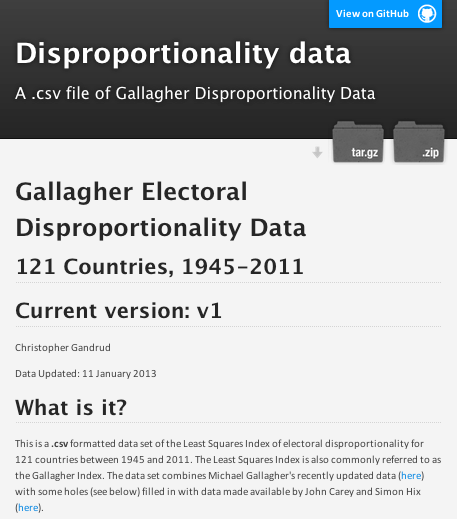
\includegraphics[width=0.45\textwidth]{images/Pages.png}
\end{center}

\subsection{Collaboration}

Compared to the status quo social science data storage methods, GitHub is uniquely strong for enabling and incentivizing collaboration both between coauthors and non-coauthors who may be able to help develop and verify the data set.  

\paragraph{Coauthors}

Public repositories can have an unlimited number of what GitHub calls ``collaborators".\footnote{To add collaborators to a repository go to its webpage and click \texttt{Settings} \textrightarrow \texttt{Collaborators} and add the coauthors' GitHub usernames.} Collaborators have permission to push changes to the repository. There is one important practical issue to note. If multiple collaborators are actively working on a data set, they need to add an extra step to their GitHub commit process.\footnote{This is also true if you make changes to both the GitHub version of the repository and the copy on your computer.} Each person needs to \texttt{pull} their collaborator's changes and resolve any merge conflicts before pushing committed changes to GitHub. Here is an example:

\begin{knitrout}
\definecolor{shadecolor}{rgb}{0.969, 0.969, 0.969}\color{fgcolor}\begin{kframe}
\begin{verbatim}
# Add new files to Git
git add .

# Commit the changes
git commit -a -m "A message"

# Pull collaborator's commits
git pull

# Push changes to GitHub
git push origin master
\end{verbatim}
\end{kframe}
\end{knitrout}


\paragraph{Collaborating with non-Coauthors: Pull requests}

People who want to make changes to a repository, but are not collaborators can make ``pull requests". All they need are GitHub accounts. Pull requests are specific changes that non-collaborators suggest. Requesters can add comments about why they are suggesting a change. GitHub also has a discussion forum where anyone can discuss these comments. 

After a pull request has been made it is up to the repository's collaborators to decide whether or not to accept the requested changes. If a collaborator accepts the changes, they are made instantly and a full record of who made the changes is kept.

There are two ways to make a pull request. If someone notices a small error--e.g. a misspelling, a misclassification--or other improvement that they think should be made to a data set, they can make a pull request by navigating to the GitHub page for the specific file they think needs to be changed. Then they click the \texttt{Edit} button located next to the \texttt{Raw} button (see above). Clicking this button ``forks" the repository, i.e. gives them a copy they can change. A record of the fork is created on GitHub. Requesters will then see  window like this:

\begin{center}
	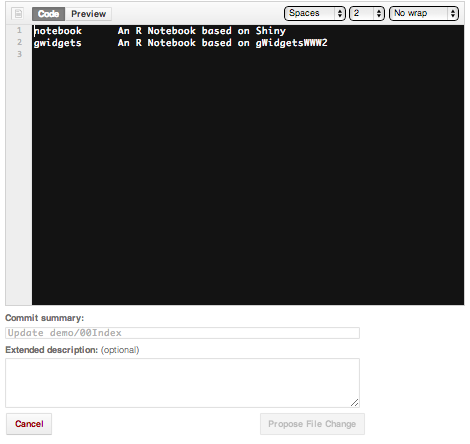
\includegraphics[width=0.46\textwidth]{images/PullRequest.png}
\end{center}

\noindent In this window they can make their proposed changes and add a comment about what the changes are and why they should be made before clicking \texttt{Propose File Change}.

For longer file changes, e.g. a major addition to the data set to bring it up-to-date, it is better to work with the forked repository rather than in the Edit window. To directly fork a data set's repository click the \texttt{Fork} button on the upper right corner of its webpage. You can then make changes to the forked repository as if it were your own. When you are ready to suggest the changes be included, you click the \texttt{Pull Request} button at the top center of the forked repository's GitHub page. For more information on forking and pull requests see the GitHub article on the topic: \url{https://help.github.com/articles/using-pull-requests}.

\paragraph{Issues}

GitHub repositories also have an ``Issues" area that allows any other GitHub user to make a comment on the repo. These tend to be general suggestions for how to improve the files or questions about the repo that may be of general interest. Anyone can respond in the Issues area creating a discussion thread.

\paragraph{Repo Wiki}

GitHub provides a very easy tool for creating nicely formatted repository wikis. For example, a data set repo's wiki could include short articles with details about how the data set was created and what it has been used for. Non-official collaborators can add to repo wikis. Like pull requests, these changes are subject to approval by one of the repository's collaborators.

\paragraph{Follow a repository}

If you are a GitHub member you can follow a public repository, even if you aren't a collaborator, This gives you a Facebook-style newsfeed\footnote{See: \url{https://www.facebook.com/help/327131014036297/}.} showing any updates made to the repository as well as discussions in the Issues area and pull requests. 

\paragraph{Passing on the data set}

Because of changing time commitments, professional interests, and so on, no one can maintain and update a data set forever. GitHub makes it easy to pass on control of a data set while maintaining it's entire version history. Simply add the new data set maintainer as a collaborator. They will largely have the same privileges to manage the repository as you did. To completely transfer control simply have the new maintainer fork the repository and leave a link to the forked version at the previous location on GitHub. Forked repositories contain the entire commit history of the original repository.

\paragraph{Selective incentives}

Why would people actively contribute to improving publicly available data sets, especially data sets primarily associated with other authors? What's in it for them? 

GitHub not only provides technology--particularly pull requests--for social data development and verification, but it also gives Olsonian selective incentives that can motivate people to do so \citep{Olson1965}. By keeping track of who made what change and providing numerous ways to quantify and visualize each member's contributions it provides strong selective incentives to collaborate. Perhaps one day social scientists could bring GitHub's descriptive statistics of their contributions, like the one below, to hiring and promotion committees.   

\begin{center}
    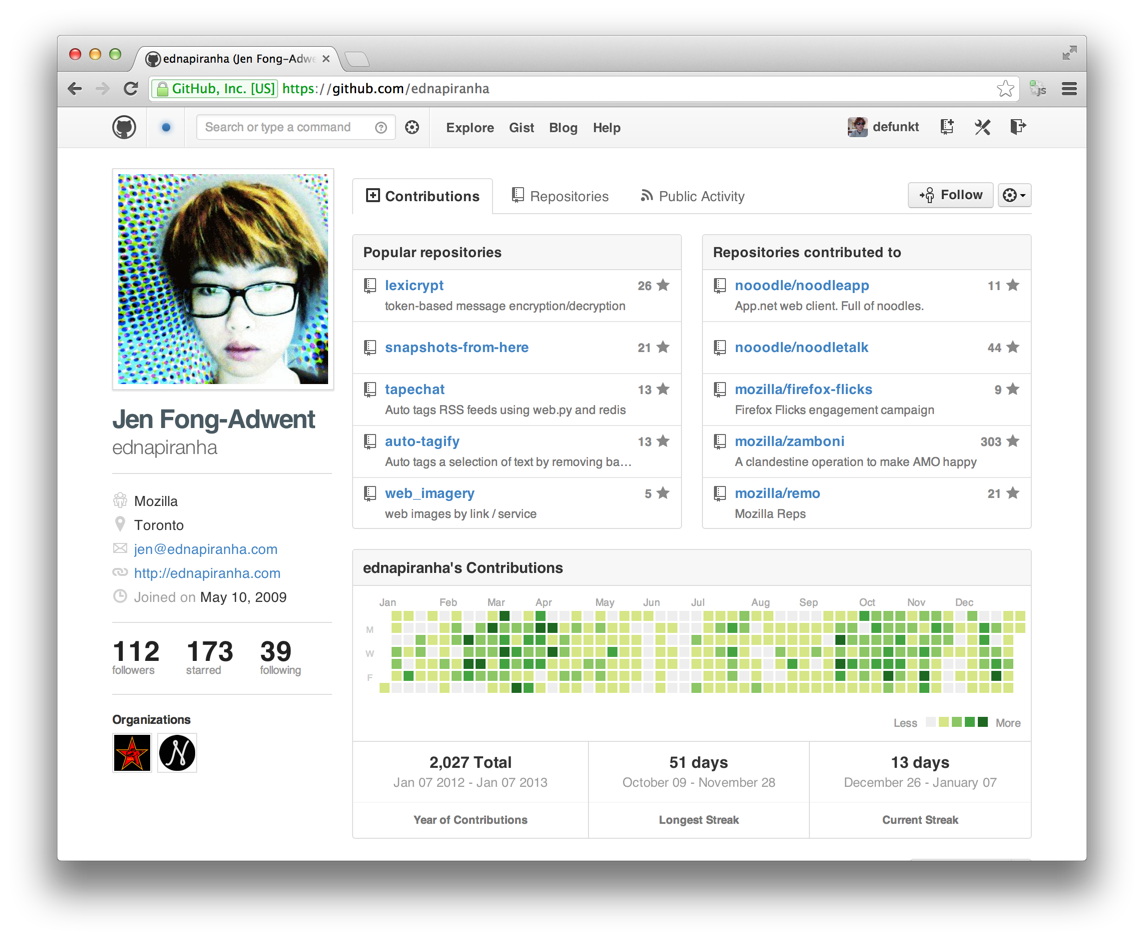
\includegraphics[width=0.46\textwidth]{images/Contributors.png}
    {\tiny{Image from \cite{Palmer2013}}}
\end{center}

\section{Conclusion}

In this article I have tried to show that GitHub is a very good option for storing actively developed original social science data in the cloud. Admittedly, it has more of a learning curve than the incumbent options. Journals wishing to host complete replication data sets for findings that they publish in a way that easily secures authorization and legal protection may want to continue to require data snapshots be deposited in a Dataverse-type archive.\footnote{Enterprising journals could create GitHub organization accounts. This would require some more work to apply the appropriate legal protections as they are not `in the box'.}

However, I hope to have demonstrated that GitHub is worth learning and using for developing and maintaining original social science data. It is at least as good as the alternatives in terms of stable storage, access, version control, and collaboration. In addition it is far better at enabling social data development and verification. GitHub has already enabled significant contributions to open source software development. We can easily use this service to both make social science data set collaboration easier and provide selective incentives to do so. Hopefully, this will improve the social science community's utilization of its collective knowledge to create more complete and robust data sets. Better data sets will allow us to better answer our research questions.




\bibliographystyle{apsr}
\bibliography{PoliSciGitStore}

\end{document}
